%%%%%%%%%%%%%%%%%%%%%%%%%%%%%%%%%
%converted dpele to dc-tpcelec
\section{System Overview}
\label{sec:dp-tpcelec-overview}

%%%%%%%%%%%%%%%%%%%%%%%%%%%%%%%%%
\subsection{Introduction}
\label{ssec:dp-tpcelec-intro}


The aim of the \dword{dp} TPC electronics is to collect and digitize the signals from the %Charge Readout Planes 
\dwords{crp} (see chapter~\ref{ch:fddp-CRP}) and \dwords{pds} (see chapter~\ref{ch:fddp-pd}), which implements %\dwords{pd}, 
\dwords{pmt}. %, in the \dword{dpmod}. 
These two tasks are respectively accomplished by the \dword{cro} and \dword{lro} sub-systems.
%\fixme{something about its components: e.g., This system comprises a \dword{cro} to read out the \dwords{crp} (see chapter xyz) and a \dword{lro} to read out the \dwords{pmt} (see chapter xyz).}
%\fixme{Also, if we have the TPC electronics ``system'' do we want the CRO and LRO ``subsystems''?}
The design of the system incorporates the components already developed for \dword{pddp} as a result of an R\&D activity started in 2006. One of the key objectives of this R\&D program has been the design of an electronics system that is easily scalable and cost-effective in order to meet the needs of the large-scale neutrino \dword{lar} detector.  %\dword{dpmod}. % neutrino \dword{lar} detector. <-The R&D was for both SP and \dual electronics  
%\fixme{you need a figure here - schematic maybe - showing the CRO and LRO system and how it fits in with the other systems (anne)} DONE

While a single \dword{dpmod} has a factor of \num{20} more readout (both charge and light) channels than \dword{pddp}, a simple scaling of the number of the components used in the prototype design is sufficient to meet these needs without necessitating any additional R\&D. A small-scale version of the TPC electronics system was used in the \dword{wa105} at CERN, a preliminary \dual \lartpc prototype with an active volume  of \SI[product-units=power]{3x1x1}{m} (\dword{crp} area of \SI[product-units=power]{3x1}{m}) that took data in the summer-fall of 2017. %The experience gained from the \dword{wa105} operation allowed to validate already some of the design choices and check various performance markers (e.g., noise). 
Operation of the \dword{wa105} validated the design choices and provided checks on various performance markers, e.g., noise. 

\begin{dunefigure}[Schematic layout of the \dword{dp} \dword{cro} sub-system]{fig:dp-tpcelec-crosystem-sketch}
{Schematic layout of the \dword{dp} \dword{cro} sub-system.}
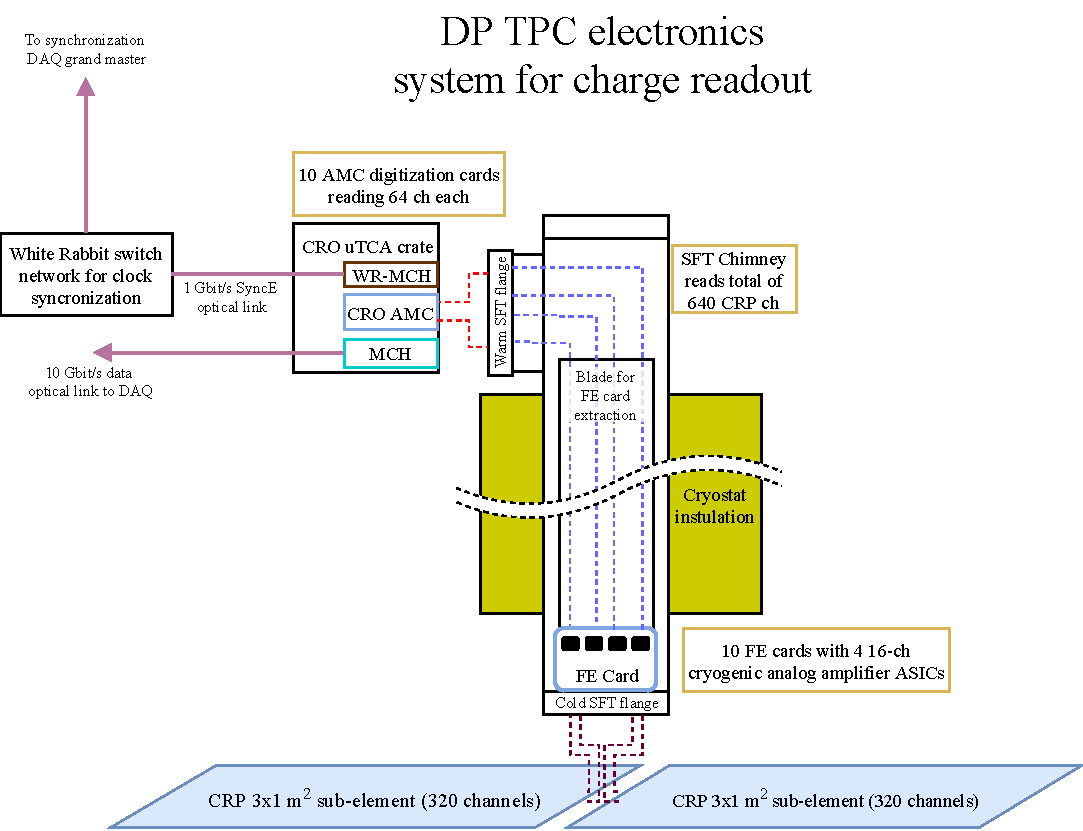
\includegraphics[width=0.6\textwidth]{dp-tpcelec-crosystem-sketch}
\end{dunefigure}

The \dword{cro} electronics system, illustrated in the Figure~\ref{fig:dp-tpcelec-crosystem-sketch}, is designed to provide continuous, non-zero-suppressed, and losslessly compressed digital signals by reading the charge collected on the \dwords{crp}' \SI{3}{m} long strips that are arranged in two collection views, all with a pitch of \SI{3.125}{mm}.% in the \dword{crp}. 
The system consists of %a 
the \dword{fe} analog electronics operating at cryogenic temperatures and digital electronics working in the warm environment outside of the cryostat.  The cryogenic \dshort{fe} analog electronics is based on an application-specific integrated circuit (\dword{asic}) chip with a large dynamic range (up to \SI{1200}{fC}) to cope with the charge amplification in the \dwords{crp}. The analog \dword{fe} cards are housed in dedicated \dwords{sftchimney} and are accessible from the outside even after the \dword{dpmod} is in operation, thus removing any significant risks associated with their long-term survivability. The \dwords{sftchimney} are approximately \SI{2.3}{m} long stainless steel pipes 
%\fixme{metallic cylinders?} DONE 
that traverse the entire insulation layer of the cryostat allowing placement of the \dword{fe} electronics close to the \dwords{crp} to minimize cable capacitance (noise).  In addition, their metallic structure shields the \dword{fe} cards 
from any interference from the warm digital electronics and ambient environment. The analog signals are digitized by \dwords{amc}, which are housed in the commercial \dword{utca} crates on top of the cryostat near the \dwords{sftchimney}. 

The \dword{cro} data are sampled at the rate of \SI{2.5}{MHz} with \SI{12}{bit} resolution.  
%\fixme{both cro and lro? sounds like only cro.} DONE
This frequency, traditionally used in \lartpc experiments, is well matched to the \SI{1}{\micro\second} pulse-shaping time of the \dword{fe} electronics and the detector response times determined by the electron drift velocity in the \lar. The corresponding sampling resolution along the drift coordinate is better than \SI{1}{\mm}. 

The \dword{lro} electronics system, illustrated in the Figure~\ref{fig:dp-tpcelec-lrosystem-sketch},  collects and digitizes the signals from the \dword{pds}, which consists of \dword{tpb}-coated \num{8}\,in \dwords{pmt} (Hamamatsu\footnote{Hamamatsu\texttrademark R5912-02-mod, \url{http://www.hamamatsu.com/}.} R5912-02-mod) located beneath the TPC cathode. The \dword{lro} electronics %should 
facilitates the detection of the primary scintillation signals, which provide the absolute time reference for the interaction events. It %should 
also enables recording the light signals generated by photons from the so-called \textit{proportional scintillation component}, the light created by the electrons extracted and amplified in the gaseous phase. A fraction of this light can reach the \dwords{pmt} after traversing the entire detector volume.  
%\fixme{what light detection element is up there?} NOW EXPLAINED  
The \dword{lro} electronics, consisting of analog and digital stages, is housed in the \dword{utca} crates on top of the cryostat structure (similar to the \dword{cro} electronics). The \dword{lro} \dword{amc} card design shares a similar architecture with the \dwords{amc} for the charge readout. The \dword{lro} \dword{utca} crates are connected to specific \dword{lro} signal \fdth flanges on top of the cryostat (see chapter~\ref{ch:fddp-pd}).
%\fixme{add: similar to the \dword{cro} electronics} is housed in the \dword{utca} crates on top of the cryostat structure.  \fixme{Need to introduce these cards before comparing them to those for the CRO}

\begin{dunefigure}[Schematic layout of the \dword{dp} \dword{lro} sub-system]{fig:dp-tpcelec-lrosystem-sketch}
{Schematic layout of the \dword{dp} \dword{lro} sub-system.}
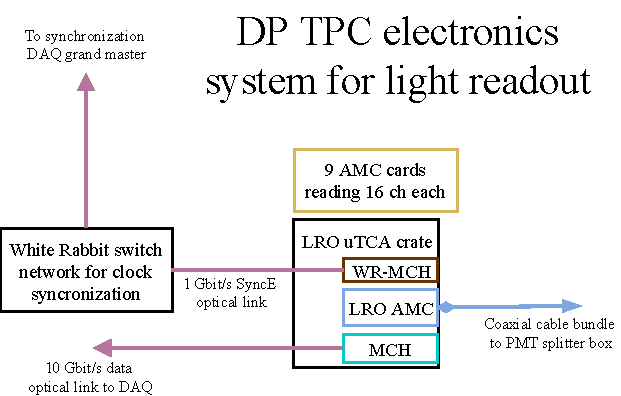
\includegraphics[width=0.6\textwidth]{dp-tpcelec-lrosystem-sketch}
\end{dunefigure}

Each \dword{utca} crate for either charge or light readout is connected to the \dword{daq} system via an optical fiber link that supports at least \SI{10}{Gbit/s}. 
%\fixme{so you dont have both LRO and CRO through same chimneys to same crates; all chimneys and crates are either one or the other?} ADDED EXPLANATION
Every crate also contains a %module, 
\dword{wrmch} for the time synchronization of the digital electronics. This timing slave unit is connected via \SI{1}{Gbit/s} optical fiber to a master node that serves as a synchronization reference for all the connected slave nodes on the network. This system for the time synchronization is based on the commercially available components developed within the framework of the \dword{wr} project\footnote{\url{https://www.ohwr.org/projects/white-rabbit}.} with ad-hoc hardware and firmware development. The system performs automatic and continuous self-calibrations to account for any propagation delays and is able to provide sub-\si{\nano\s} accuracy for the timing synchronization.



%%%%%%%%%%%%%%%%%%%%%%%%%%%%%%%%%
\subsection{Design Considerations}
\label{ssec:dp-tpcelec-requir}

%The principal requirements for the \dual TPC electronics system can be summarized as:
%\fixme{Could we separate out CRO and LRO? It feels like this goes back and forth. They really are separate, aren't they?  Maybe separate into CRO, LRO and common considerations...?  Also I think this section could be trimmed quite a bit.} THEY CANNOT BE SEPARATED SINCE LRO INHERITS THE SAME AMC ELECTRONICS. THE MOST NATURAL WAY IS TO INTRODUE THE CRO AND THEN LRO ELECTRONICS

The \dword{cro} electronics design covers the analog \dword{fe} cards containing pre-amplifier \dwords{asic} operating at cryogenic temperatures and digitization cards with the relevant system for their synchronization working in the warm environment outside of the cryostat. The system %should 
reads and digitizes signals from a total of \num{153600} channels (per one \dword{dpmod}) and is capable of continuously streaming the collected and losslessly compressed data to the \dword{daq} without any zero suppression. 
The design of the \dshort{cro} electronics system was developed to fit the following requirements:
\begin{itemize}
\item{The \dword{cro} electronics %must be able to 
must measure signals of up to \SI{1200}{\femto\coulomb} without saturation; this has been optimized following \dword{mc} studies on the maximal occupancy per channel in shower events~\cite{WA105-TDR}. For a nominal \dword{crp} gain of \num{20}, a \dword{mip} signal is expected to be around \SI{30}{fC} -- the lowest limit that assumes a particle travelling horizontally with an azimuthal angle of \num{0} degrees -- giving %the 
a maximal operational range of up to \num{40} \dwords{mip}.}

\item{The electronic noise in the \dshort{cro} analog electronics is required to be \SI{< 2500}{e^{-}}. This condition can be derived from the requirement on the minimal \dword{s/n}, which should be greater than \num{5}:\num{1} once the charge attenuation is taken into account. Given the maximum drift distance of \SI{12}{\meter}, the largest attenuation factor due to electro-negative impurities assuming the \SI{3}{\milli\second} (minimally required) electron lifetime and the drift field of \SI{0.5}{\kilo\volt/\cm} is \num{0.08}. The smallest \dword{mip} signal with the \dword{crp} effective gain of \num{20} is therefore \SI{2.5}{\femto\coulomb} (\SI{15600}{e^{-}}).}

\item{The peaking time of the \dword{fe} analog amplifiers %should 
must be \SI{1}{\micro\second}. This requirement is driven by the need for optimal vertex resolution, determined in turn by the single track resolution and the power to separate two or more tracks that are close to one another.}

\item{The sampling frequency %should 
must be \SI{2.5}{\MHz} to match the peaking time of the \dword{fe} electronics.}

\item{The power dissipated by the \dword{fe} analog electronics %must 
must be below \SI{50}{\milli\watt/channel} in order to minimize the heat input to the cryostat volume.}

\item{The \dword{fe} analog electronics %should 
must be replaceable without the risk of contaminating the main \lar volume in order to guarantee the long-term reliability of the system.}

\item{The \dword{adc} resolution %should 
must be such that the noise is at the level of an \dword{adc}
%\fixme{does not exceed?} the level of an \dword{adc}, %while THIS WAS CORRECT
given a dynamic range wide enough to match the response of the \dword{fe} amplifier. This can be achieved with a \num{12} bit \dword{adc}.}

\item{The digital electronics to be placed outside of the cryostat in the warm environment %can 
must be capable of adopting standard industrial components and solutions, to keep the costs lower and to benefit from  %ensuring low costs and benefiting of the 
technological evolution, e.g., higher network speeds.}
\end{itemize}
As described %in the details 
in subsequent sections, the achieved performance of the final system is significantly better than many of the listed requirements.  %\fixme{above sentence not clear: performance exceeds requirements? (anne)} YES, THERE WERE MINIMAL REQUIREMNTS COMING FROM EXPERIENCE WITH SP DETECTORS

The magnitude of the noise also %plays a role in 
has an effect on the quality of the lossless compression of the raw data. % performed by the digital electronics. 
A compression factor of about \num{10} is achieved with the \rms noise level below \SI{1}{\dword{adc}}. To give an idea of the compression efficiency dependency on the noise level a compression factor of four is obtained with the noise at around \SI{1.5}{\dword{adc}} counts. 
%\fixme{What are you saying here: ``we're expecting 1.5 ADC so we'll only get factor of 4, but wouldn't it be nice to get factor of 10''? If that's your meaning, what's keeping you from getting the noise low enough?} REFORMULATED THE SENTENCE
% A compression factor of \num{7} can be achieved with a \rms noise level of $\sim$ \SI{1.5}{\dword{adc}}, increasing to \num{10} for \rms noise levels below \SI{1}{\dword{adc}} \rms.

%Given the amplification of the ionization charge in \dword{crp}, the electronics needs to be sensitive to the signals over a large dynamic range (up-to \num{40} times the \dword{mip}-level signals for a nominal \dword{crp} gain of %\num{20} or \SI{1200}{\femto\coulomb}) to avoid saturation of the analog inputs by large localized energy disposition produced, for example, in shower events. The minimal requirelemt on the intrinsic noise %of the \dword{fe} analog electronics is \SI{<2500}{e^{-}}.  The condition is derived from the requirement on the minimal \dword{s/n} of \num{5:1} as in the SP design. Given the maximal drift \SI{12}{\meter} the %largest attenuation factor due to electro-negative impurities assuming the nominal \SI{3}{\milli\second} electron lifetime is \num{0.08}. The smallest \dword{mip} signal with the \dword{crp} effective gain is therefore %\SI{2.5}{\femto\coulomb} (\SI{15600}{e^{-}}).

%The charge amplification provided by the \dword{crp} loosens requirements on the intrinsic noise of the \dword{fe} analog electronics. For the \dword{crp} nominal gain of \num{20}, the signal-to-noise ratio for a \dword{mip} signal %(\SI{30}{fC}) should be around \num{100}, which would not pose any problems for the detection/reconstruction. 

The primary objective of the \dword{lro} system is to detect signals, from a minimum of one \phel on one \dword{pmt}, giving a precise timestamp that can be used in conjunction with the charge signals to determine the absolute event time ($T_0$). 
%\fixme{why insert (drift)?} MODIFIED
Precise measurements of \dword{lro} signal charge allow the continual monitoring of the \dword{pmt} gain at the single \phel level, and the determination of the number of photons in each scintillation event.  In addition, an \dword{adc}  continuously streams data, downsampled to \SI{400}{ns} as for the \dword{cro} signals,  which, amongst other items, allows measurements of the scintillation time profile. The \dword{lro} system also reads \num{20} channels from reference SiPM sensors from the \dword{pd} calibration system.
%\fixme{``...number of signals from the \dword{pd} calibration trigger and about \num{20} channels from calibration reference sensors.'' (?)} EXAPLAINED BETTER 

The cryogenic analog electronics for the \dword{cro} is housed in the dedicated \dwords{sftchimney}. %Their 
Its design %must 
enables access to the \dword{fe} card for possible replacement without %any 
risk of contaminating the pure \lar in the main cryostat volume. The chimneys %must 
possess a cooling system that can control the temperature around the \dword{fe} cards to roughly \SI{110}{\kelvin} %for their optimal noise. 
to reach their optimal noise level and %. In addition, the cooling system must 
that compensates for the heat input from the chimneys into the cryostat volume. 

The digital electronics for both charge and light readout is located in the warm environment on the top of the cryostat supporting structure and is therefore easily accessible. This fact removes any constraints associated with the accessibility and operation in cryogenic environments allowing for the usage of standard components and industrial solutions in the design. Digital electronics must be continuously and automatically synchronized to better than \SI{400}{\nano\s} to ensure the correct temporal alignment of the \dword{adc} samples from all of the readout channels. This is a minimal requirement dictated by the fact that the sampling rate is \SI{2.5}{\MHz}.  

%Some of the k
Key parameters for the electronics system design are summarized in Table~\ref{tab:dp-tpcelec-physicsparams}. %The requirements for the \dual electronics system are documented in DUNE-docdb-6428.

\begin{dunetable}
[Parameters for the TPC electronics system design]
{lr}
{tab:dp-tpcelec-physicsparams}
{Parameters for the  TPC electronics system design. The numbers are given for one \dword{dpmod}.}   
Parameter & Value  \\ \toprowrule
  \dword{cro} channels    &  \num{153600}            \\ \colhline
  \dword{cro} continuous sampling rate & \SI{2.5}{\MHz}\\ \colhline
  \dword{cro} \dword{adc} resolution & \num{12}\,bit           \\ \colhline
  \dword{cro} data compression factor   & \num{10}    \\ \colhline 
  \dword{cro} data flow  & \num{430}\,Gibit/s          \\ \colhline 
  \dword{lro} channels       & \num{720}               \\ \colhline
  \dword{lro} continuous sampling rate & \SI{2.5}{\MHz} \\ \colhline
  \dword{lro} \dword{adc} resolution & \num{14}\,bit            \\ \colhline
  \dword{lro} data compression factor  & \num{1}       \\ \colhline
  \dword{lro} data flow   & \num{24}\,Gibit/s          \\ 
\end{dunetable}
%\fixme{Gibit instead of Gbit?} YES, SINCE THEN NUMBERS WERE COMPUTED IN THE BASE OF 1024, CHECKED WITH BRETT



%%%%%%%%%%%%%%%%%%%%%%%%%%%%%%%%%
\subsection{Scope}
\label{ssec:dp-tpcelec-scope}


The scope of the TPC electronics system covers the procurement, production, testing, validation, installation, and commissioning of all the components necessary to ensure the complete readout of the charge and light signals from a given \dword{dpmod}. This includes: %The covered items are the following:
\begin{itemize}
\item{Cryogenic analog \dword{fe} cards for charge readout;}
\item{\dword{amc} cards for charge and light readout;}
\item{The \dword{wrmch} cards for \dword{amc} clock synchronization;}
\item{\dword{utca} crates;}
\item{Switches for the \dword{wr} network;}
\item{\dwords{sftchimney};}
\item{Low-voltage power supplies, distribution, and filtering system for the \dword{fe} cards;}
\item{Flat cables connecting the \dword{fe} cards to the warm flange interface of the \dwords{sftchimney};}
\item{VHDCI cables connecting the warm flange interface of the \dwords{sftchimney} to \dwords{amc}.}
\end{itemize}

%\fixme{what about cables/connections to the \dwords{crp} and \dwords{pmt}?} THEY ARE PROVIDED BY OTHER CONSORTIA AS COVERED IN THE INTERFACE SECTION

The total numbers for components to be procured to instrument one \dword{dpmod} are given in Table~\ref{tab:dp-tpcelec-num-components}

\begin{dunetable}
[Numbers for \dual electronics components to procure]
{lr} {tab:dp-tpcelec-num-components}
{Numbers for \dual electronics components to procure for one \dword{dpmod}.}
Name & Number  \\ \toprowrule
\dword{cro} cryogenic \dwords{asic} (\num{16} ch) & \num{9600} \\ \colhline
\dword{cro} cryogenic analog \dword{fe} cards (\num{64} ch) & \num{2400} \\ \colhline
\dword{cro} \dwords{amc} & \num{2400} \\ \colhline
\dwords{sftchimney} & \num{240} \\ \colhline
Flat cables for \dword{sftchimney} (\num{68} ch) & \num{2400} \\ \colhline
Flat cables for \dword{sftchimney} (\num{80} ch) & \num{2400} \\ \colhline
VHDCI cables (\num{32} ch) & \num{4800} \\ \colhline
\dword{lro} \dwords{amc} with analog \dword{fe} & \num{45} \\ \colhline
\dword{utca} crates & \num{245} \\ \colhline
\dword{wrmch} units & \num{245} \\ \colhline
WR switches (\num{18} ports) & \num{16} \\ 
\end{dunetable}

